% Macros and configuration for this chapter
\lstdefinelanguage[]{Coq}[]{}{literate=%
{>}{{$>$}}{1}
{<}{{$<$}}{1}
{=}{{$=$}}{1}
{-}{{$-$}}{1}
{+}{{$+$ }}{1}
{~}{{$\sim$}}{1}
{===}{$\equiv$ }{1}
{...}{$\ldots$ }{2}
{<--}{\reflectbox{$\leadsto$}}{3}
{->}{$\rightarrow$ }{1}
{=>}{$\Rightarrow$ }{1}
{>=}{$\ge$}{1}
{<=}{$\le$}{1}
{:=}{$\coloneqq$}{2}
{/\\}{{$\wedge$}}{1}
{\\/}{{$\vee$}}{1}
{forall}{$\forall$}{1}
{TTrue}{{True}}{4}
{FFalse}{{False}}{5}
{True}{{$\top$}}{1}
{False}{{$\bot$}}{1}
%{'a}{{$\alpha$}}{1}
%{'b}{{$\beta$}}{1}
%{'c}{{$\gamma$}}{1}
%{'d}{{$\delta$}}{1}
%{'e}{{$\varepsilon$}}{1}}
,
morekeywords={Inductive,Definition,Fixpoint,Lemma,Theorem,Proof,Qed,Require,Import,Set,Type,Prop,match,fun,apply,intros,exact,destruct,split,simpl,reflexivity,exfalso,induction,rewrite,left,right}
}
\lstdefinestyle{Coq}{language=Coq}
\lstset{style=Coq}

\lstdefinelanguage[]{Coqorig}[]{}{literate=%
{>}{{$>$}}{1}
{<}{{$<$}}{1}
{=}{{$=$}}{1}
{-}{{$-$}}{1}
{+}{{$+$ }}{1}
% {~}{{$\sim$}}{1}
{===}{$\equiv$ }{1}
{...}{$\ldots$ }{2}
{<--}{\reflectbox{$\leadsto$}}{3}
{->}{$\rightarrow$ }{1}
{=>}{$\Rightarrow$ }{1}
{>=}{$\ge$}{1}
{<=}{$\le$}{1}
{:=}{$\coloneqq$}{2}
{/\\}{{$\wedge$}}{1}
{\\/}{{$\vee$}}{1}
{forall}{$\forall$}{1}
% {~}{{$¬$}}{1}
%{'a}{{$\alpha$}}{1}
%{'b}{{$\beta$}}{1}
%{'c}{{$\gamma$}}{1}
%{'d}{{$\delta$}}{1}
%{'e}{{$\varepsilon$}}{1}}
,
morekeywords={Inductive,Definition,Fixpoint,Lemma,Theorem,Proof,Qed,Require,Import,Set,Type,Prop,match,fun,apply,intros,exact,destruct,split,simpl,reflexivity,exfalso,induction,rewrite,left,right}
}
\lstdefinestyle{Coq}{language=Coq}
\lstset{style=Coq}

\chapter{Theorem Proving}
\label{chap_theorem}

\targets{
  \item \textit{Programming}: By using Recursive Functions and Inductive Data Types
  \item \textit{Specifying}: Understand how Logical Formulas can be encoded as Types
  \item \textit{Proving}: Prove Logical Formulas about Programs in the interactive theorem prover Coq
}

% !TeX root = ../../presentation-local.tex

\section{Introduction}

\begin{frame}{(Again) Using Logic for Verification}
\begin{itemize}
	\item Consider
	\begin{itemize}
		\item \textbf{Program} $P$ of type $ℕ \times ℕ \rightarrow ℕ$ that does something interesting... like adding two numbers!
		\item \textbf{Specification} $\phi$: For every input $m, n$ the terms $P(m, n)$ and $P(n, m)$ should reduce to the same value (\say{commutativity})
	\end{itemize}

	\pause

	\item $P$ and $\phi$ must be describable in the logic
	\begin{align*}
		\phi_P &:= ∀ m, n.~ \left(\begin{aligned}
			  P(0, n)   &\succ n\\
			∧~ P(S~m, n) &\succ S(P(m, n))
		\end{aligned}\right)\\[1em]
		\phi &:= ∀ m, n.~∃ x.~ P(m, n) \succ^{*} x ∧ P(n, m) \succ^* x
	\end{align*}

	\pause

	\item $\succ$ denotes \textit{term reduction}, but different computation models could be described, e.g. transitions on Kripke structures, manipulations of stack machines, memory transformations...

\end{itemize}
\end{frame}

\begin{frame}{(Again) Using Logic for Verification}
	\begin{align*}
		\phi_P &:= ∀ m, n.~ \left(\begin{aligned}
			  P(0, n)   &\succ n\\
			∧~ P(S~m, n) &\succ S(P(m, n))
		\end{aligned}\right)\\[1em]
		\phi &:= ∀ m, n.~∃ x.~ P(m, n) \succ^{*} x ∧ P(n, m) \succ^* x
	\end{align*}
~\\[1.5em]
\begin{itemize}

	\item We want to \textbf{verify}: Is $P$ correct with respect to $\phi$?
	\item In logical terms: Is formula $φ_P → φ$ \textbf{valid}?
	\begin{itemize}
		\item What does \say{valid} mean again? Recap on next slide!
	\end{itemize}

\end{itemize}
\end{frame}

\begin{frame}{Start simple: Propositional Logic}
\begin{itemize}
	\item Syntax
	\begin{itemize}
		\item Formulas $\phi, \psi := p \in AP~|~ ⊥ ~|~ \phi \rightarrow \psi$
		\item Atomic propositions $AP$
		\item (further connectives $\neg, ∧, ∨, ...$ can be used as notation)
	\end{itemize}

	\pause

	\item Semantics
	\begin{itemize}
		\item Truth domain $T := \{0, 1\}$
		\item Interpretations $v \in AP \rightarrow T$
		\item Evaluation function
		\begin{align*}
		\llbracket p \rrbracket_v &:= v(p)\\
		\llbracket ⊥ \rrbracket_v &:= 0\\
		\llbracket \phi \rightarrow \psi \rrbracket_v &:= \left\{\begin{aligned}
			1 & \quad\text{if $\llbracket \phi \rrbracket_v = 0$ or $\llbracket \psi \rrbracket_v = 1$}\\
			0 & \quad\text{otherwise}
		\end{aligned}\right.
		\end{align*}
		\item~\\[-1em]
		\begin{tabular}{l r @{\qquad}l}
		Satisfaction          & $v \vDash \phi$ & $:\Leftrightarrow \quad \llbracket \phi \rrbracket_v = 1$ \\
		Validity              & $\vDash \phi$   & $:\Leftrightarrow \quad v \vDash \phi ~~\text{for all $v$}$ \\
		\end{tabular}
		\item $φ$ is called a tautology if $\vDash \phi$
	\end{itemize}
\end{itemize}
\end{frame}

\begin{frame}{Why \textit{proving}?}
\begin{itemize}
	\item Goal: Given $\phi$, does $\vDash \phi$ hold?
	\item First approach:
	Evaluate and check $\llbracket \phi \rrbracket_v = 1$ for all $v$

	\pause

	\item Problem:
	\begin{itemize}
		\item for Propositional Logic: Possible, but there are $2^n$ interpretations (where $n$ is the number of vars in $\phi$)
		\item for First-Order Logic: Impossible, there may be \textbf{infinitely} many interpretations
	\end{itemize}

	\pause

	\item Help:
	\begin{itemize}
		\item Use a proof system
		\item Idea: Construct a \textbf{finite} proof that $φ$ holds\\[1em]
		\item Proof system must be \textit{sound}: \\
		If $\phi$ can be proven ($\vdash \phi$), then $\phi$ is valid \hspace{3.1em}($\vDash \phi$)\\[1em]
		\item Proof system \textit{may} be \textit{complete}:\\
		If $\phi$ is valid \hspace{2.8em} ($\vDash \phi$), then $\phi$ can be proven ($\vdash \phi$)
	\end{itemize}
\end{itemize}
\end{frame}

\begin{frame}{Proof System for Propositional Logic}
\begin{itemize}
\item Natural deduction via entailment relation $Γ ⊢ φ$
\begin{itemize}
	\item $Γ$ is a finite set of formulas $ψ_1, ψ_2, ..., ψ_n$
	\item \say{from $Γ$, one can \textbf{deduce} $φ$}
\end{itemize}

\pause

\item Defined by inference rules:\\
{\footnotesize
\begin{align*}
&
\inferrule*[left={\footnotesize$φ ∈ Γ$},right=Assump]
{
	~
}
{
	Γ ⊢ φ
}
%
\qquad
%
&&
\inferrule*[right=DoubleNeg]
{
	Γ, (φ \rightarrow ⊥) ⊢  ⊥
}
{
	Γ ⊢ φ
}
%
\\[1em]
%
&
\inferrule*[right=ImpIntro]
{
	Γ,ψ ⊢ φ
}
{
	Γ ⊢ ψ \rightarrow φ
}
%
\qquad
%
&&
\inferrule*[right=ImpElim]
{
	Γ ⊢ ψ \rightarrow φ\\
	Γ ⊢ ψ
}
{
	Γ ⊢ φ
}
\end{align*}}~\\

\pause

\item This system is \textit{sound}:\\
If $\phi$ can be proven ($\vdash \phi$), then $\phi$ is valid ($\vDash \phi$)
\item This system is \textit{complete}:\\
If $\phi$ is valid ($\vDash \phi$), then $\phi$ can be proven ($\vdash \phi$)
\end{itemize}
\end{frame}

\begin{frame}{Proof Trees}
\begin{itemize}
\item Check validity of $φ := p \rightarrow (q \rightarrow p)$

\pause

\item Prove $⊢ φ$ by the following proof tree
$$
\inferrule*[Right=ImpIntro]
{
	\inferrule*[Right=ImpIntro]
	{
		\inferrule*[left={\footnotesize$p ∈ \{p, q\}$},Right=Assump]
		{ }
		{p, q ⊢ p}
	}
	{p ⊢  q \rightarrow p}
}
{⊢ p \rightarrow (q \rightarrow p)}
$$

\pause

\item By soundness of $⊢$, $φ$ is valid
\end{itemize}
\end{frame}

\begin{frame}{Proof Trees in Type Systems, 1}
\begin{itemize}
	\item In a typed programming language, we want to check that $t$ is a term of type $T$

	\pause

	\item Terms
	\begin{itemize}
		\item $3+2$
		\item $\mathit{if}~\mathit{true}~\mathit{then}~\mathit{true}~\mathit{else}~\mathit{false}$
		\item $λn.n$
		\item $λn.~(λb.~\mathit{if}~b~\mathit{then}~n~\mathit{else}~n+n)$
	\end{itemize}

	\pause

	\item Types
	\begin{itemize}
		\item $\mathit{Int}$
		\item $\mathit{Bool}$
		\item $\mathit{Int}→\mathit{Int}$
		\item $\mathit{Int} → (\mathit{Bool} → \mathit{Int})$
	\end{itemize}

	\pause

	\item We write $⊢ t: T$ if term $t$ has type $T$
\pause

\item \textit{Side note}: A type system is sound if $⊢ t: T$ implies that $t$ won't \say{crash} on execution. E.g., \lstinline|true| + 4 crashes
\end{itemize}
\end{frame}

\begin{frame}{Proof Trees in Type Systems, 2}
\begin{itemize}

\item To check whether $t := λx. (λy. x)$ is of type $T := \mathit{Int} → (\mathit{Bool} → \mathit{Int})$, we check whether there is a proof tree for $⊢ t: T$

\pause

\item For our example, there is:
$$
\footnotesize
\inferrule*[Right={\footnotesize Abs}]
{
	\inferrule*[Right={\footnotesize Abs}]
	{
		\inferrule*[left={\footnotesize$(x: \mathit{Int}) ∈ \{x: \mathit{Int}, y: \mathit{Bool}\}$},right={\footnotesize Env}]
		{ }
		{x: \mathit{Int}, y: \mathit{Bool} ⊢ x: \mathit{Int}}
	}
	{x: \mathit{Int} ⊢ λy. x : \mathit{Bool} → \mathit{Int}}
}
{⊢ λx. (λy. x): \mathit{Int} → (\mathit{Bool} → \mathit{Int})}
$$

\pause

\item In a type system, the inference rules are designed s.t. for every pair $⊢ t: T$, there exists \textbf{at most one} proof tree

\pause

\item $t$ itself witnesses its own proof tree of $⊢ t: T$

\pause

\item \textit{Intuition}: A term itself represents a syntax tree. Put this tree upside down. Traverse the tree, thereby annotating types according to the inference rules. If this works out, you have \textbf{the} proof tree. Otherwise, there is none.


\end{itemize}
\end{frame}



\begin{frame}{Preview: Type System as a Proof System}
\begin{itemize}
\item You noticed the similarity between the two proof trees?
\item Is it be possible to encode a proof tree for a logic as a proof tree for a type system?

\pause

\item It is possible. It has been discovered in 1980 by Howard (Curry-Howard-Correspondence)

\pause

\item What do we need?
  \begin{enumerate}
		\item Goal: Find a way of \textit{proving} a specification $\phi$
		\item We encode $\phi$ as a type $T$
		\item We find a term $t$ that is well-typed, i.e. $⊢ t: T$
		\item But this means that $t$ witnesses a proof tree for $T$
		\item Thus we interpret $t$ as a proof of $T$ and therefore of $φ$!
  \end{enumerate}
\end{itemize}
\end{frame}


\begin{frame}{Interactive Theorem Provers}
\begin{itemize}
	\item Proofs are \textbf{manually written}, potentially with some automatic proof-search aid
	\item Proofs are \textbf{completely formal}
	\item Proofs can be \textbf{automatically checked}
	\item You have to trust in the soundness of the proof checker
		\begin{itemize}
			\item Trust is usually established by providing a minimal base of the proof checker
		\end{itemize}

	\pause

	\item Examples: Coq, Isabelle, Agda
	\item May be based on type theory, but not necessarily
	\item Applications
	\begin{enumerate}
		\item Formalized Mathematics, e.g. Four-color theorem in 1976
		\item Correctness Properties
		  \begin{itemize}
			\item Certified C compiler CompCert, started in 2005
			\item Soundness of type systems
			\item Correctness of protocols
			\item Further theorems about formalisms
		  \end{itemize}
		\item Generally: Verification where the system model or the property is \say{too complex} for automatic methods
	\end{enumerate}
\end{itemize}
\end{frame}

% !TeX root = ../../presentation-local.tex

\section{Coq Programming}

\begin{frame}{Coq}
\begin{itemize}
  \item Coq is an interactive theorem prover
  \item Main idea: Propositions as Types, Proofs as Terms (Curry-Howard-Correspondence)
  \item One can define
    \begin{itemize}
      \item Inductive \textbf{Types (Propositions)}
      \item Well-typed \textbf{Terms (Proofs)}
    \end{itemize}
  \item The underlying language Gallina
    \begin{itemize}
      \item is a dependently-typed functional programming language
      \item implements the Calculus of Inductive Constructions
      \item is not Turing-complete (every term has a normal form)
    \end{itemize}
\end{itemize}
\begin{center}
  
\includegraphics[width=0.33\textwidth]{content/theorem-proving/images/coq.png}
\end{center}
\end{frame}

\begin{frame}{Getting started with Coq}
\begin{enumerate}
  \item Installation
    \begin{itemize}
      \item Win/Mac: Download from \url{https://coq.inria.fr/}
      \item Linux: We recommend installation via OPAM \url{https://coq.inria.fr/opam/www/using.html}
    \end{itemize}
  \item IDE
    \begin{itemize}
      \item Recommendation: Coq IDE, shipped with Coq (see screenshot)
      \item Popular plugin for Emacs: Proof General
    \end{itemize}
\end{enumerate}
\begin{center}
  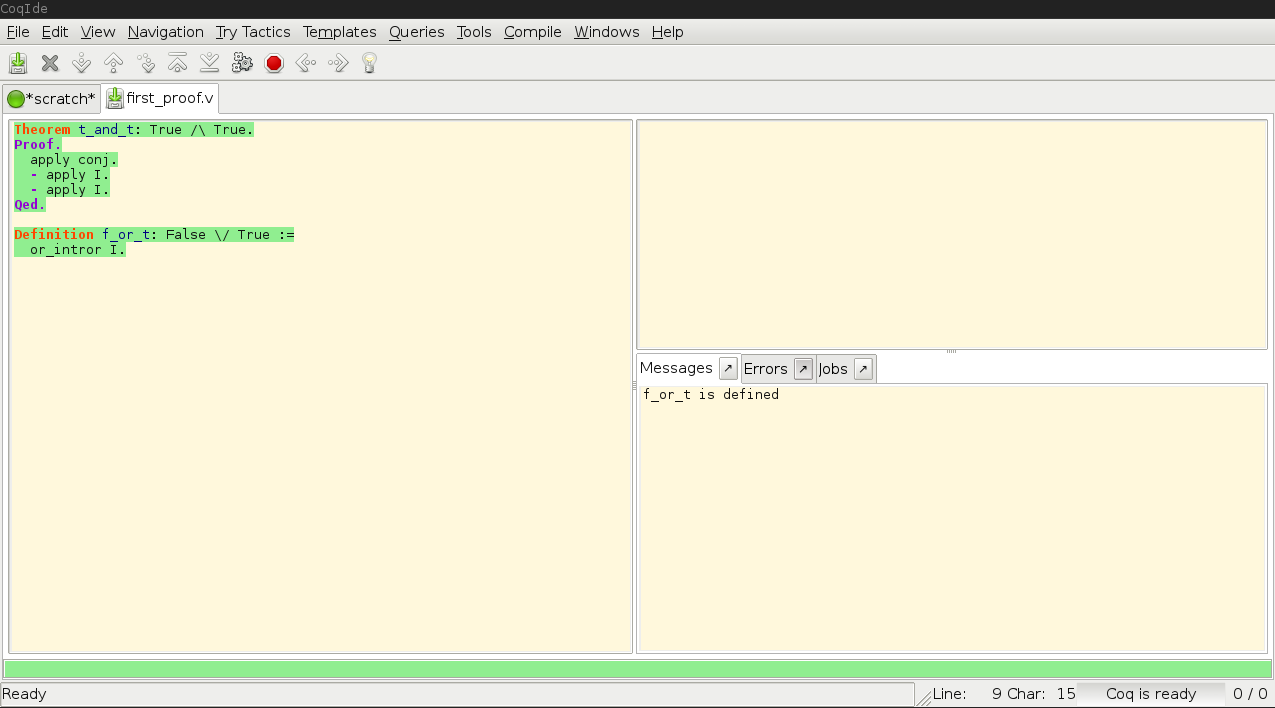
\includegraphics[width=0.8\textwidth]{content/theorem-proving/images/coqide.png}
\end{center}
\end{frame}

\begin{frame}[fragile]{Coq Programming\small~~ (Inductive Data Types)}
\begin{itemize}
  \item An inductive data type definition introduces a \textbf{new type} and \textbf{new well-typed terms}
\lstinputlisting{content/theorem-proving/coq/snippets/bool_nat.v}

\pause

\item \lstinline|bool|, \lstinline|nat| are types
\item \lstinline|true|, \lstinline|false|, \lstinline|O|, \lstinline|S| are value constructors
\end{itemize}
\end{frame}

\begin{frame}[fragile]{Coq Programming\small~~ (Definitions)}
\begin{itemize}
  \item A \lstinline|Definition| gives a name to a term
  \lstinputlisting{content/theorem-proving/coq/snippets/three.v}

  \pause

  \item Definitions can be unfolded, which is a kind of \textit{reduction}

  \item Two terms are \textit{convertible} ($\equiv$) if they reduce to the same term

  \item The terms \lstinline|S two| and \lstinline|three| are convertible
\begin{lstlisting}
  S two
=== S(S(S O))
=== three
\end{lstlisting}

  \pause

  \item \textit{Intuition:} Convertibility is \say{syntactic equality up-to certain manipulations}
\end{itemize}
\end{frame}

\begin{frame}[fragile]{Coq Programming\small~~ (Functions, Pattern Matching)}
\begin{itemize}
  \item We can define functions that use pattern matching
  \lstinputlisting{content/theorem-proving/coq/snippets/negb.v}

  \pause

  \item \lstinline|fun x => ...| introduces a function
  \item \lstinline!match ... with | ... end! pattern-matches

  \pause

  \item Both constructs introduce a form of reduction and thus of convertibility
\begin{lstlisting}
  negb true
=== (fun x => ...) true
=== match true with | true => false | ...
=== false
\end{lstlisting}
\end{itemize}
\end{frame}

\begin{frame}[fragile]{Coq Programming\small~~ (Short Notation for Functions)}
\begin{itemize}
  \item Recall our function
  \lstinputlisting{content/theorem-proving/coq/snippets/negb.v}
  \item We can use the following short notation
  \lstinputlisting{content/theorem-proving/coq/snippets/negb_param.v}
\end{itemize}
\end{frame}

\begin{frame}[fragile]{Coq Programming\small~~ (Type-Checking)}
\begin{itemize}
  \item In Coq, every term must be well-typed
  \item What does that mean?
  \begin{itemize}
    \item We write $Γ ⊢ t: T$ and call it a \textit{(typing) judgement}
    \item \say{Under context $Γ$, term $t$ has type $T$}
    \item Context $Γ$ is a list of items $t: T$
    \item ~\\[-3em]
    \begin{alignat*}{2}
      \text{E.g., we have} &\quad x: \mathit{bool} ~&⊢ \mathit{negb}~x: \mathit{bool}\\
      \text{...but \textbf{not}} &\quad x: \mathit{nat} ~&⊢ \mathit{negb}~x: \mathit{bool}
    \end{alignat*}
  \end{itemize}

  \pause

  \item Coq can \textit{try to find} a type $T$ for $Γ, t$ (a.k.a. \textbf{type inference}, generally undecidable)

  \pause

  \item Coq \textit{decides} for a given judgement whether it holds (a.k.a. \textbf{type-checking})
\end{itemize}
\end{frame}

\begin{frame}[fragile]{Coq Programming\small~~ (Type-Checking, Reducing in Coq)}
\begin{itemize}
  \item Type-infer terms and compute (reduce) terms
\begin{lstlisting}[mathescape=true]
Check (negb true).   $\leadsto$  negb true: bool
Compute (negb true). $\leadsto$  false: bool
\end{lstlisting}
  \begin{itemize}
    \item Here, the context $Γ$ is considered by Coq but not explicitly output
  \end{itemize}
\end{itemize}
\end{frame}

\begin{frame}[fragile]{Coq Programming\small~~ (Recursive Functions)}
\begin{itemize}
  \item We can define recursive functions
  \lstinputlisting{content/theorem-proving/coq/snippets/plus_param.v}

  \pause

  \item Above was really a short notation for the following:
  \lstinputlisting{content/theorem-proving/coq/snippets/plus.v}
\end{itemize}
\end{frame}

\begin{frame}[fragile]{Coq Programming\small~~ (Recursion must be structural)}
\lstinputlisting{content/theorem-proving/coq/snippets/plus_param.v}
\begin{itemize}
  \item Recursive functions in Coq \textbf{always terminate} because only \textit{structural recursion} is allowed

  \pause

  \item Structural recursion means that recursion is only applied to sub-structures
  \item Here: \lstinline|m'| is a sub-structure of \lstinline|S m'|

  \pause

  \item Why this restriction? Remember: Proofs are programs, and non-terminating proofs must be avoided!\\
  (more later)
\end{itemize}
\end{frame}

\begin{frame}{Coq Programming\small~~ (Prelude and Notation)}
\begin{itemize}
  \item Standard data types, functions, notation are pre-defined via the Prelude\footnote{\scriptsize\url{https://coq.inria.fr/library/Coq.Init.Prelude.html}}
  \item This allows us to write a term like \lstinline|3 + 2| instead of \lstinline|plus S(S(S O)) S(S O)|.
  \item We use the nice notation from now on wherever possible
\end{itemize}
\end{frame}

\begin{frame}[fragile]{Coq Programming\small~~ (Polymorphic Data Types, 1)}
\begin{itemize}
  \item It is often useful to parameterize a data type to avoid multiple definitions such as \lstinline|natList|, \lstinline|boolList| etc.
\lstinputlisting{content/theorem-proving/coq/snippets/list_param.v}

  \pause

  \item We say that \lstinline|list| is \textit{polymorphic} in its \textit{parameter} \lstinline|X|

  \pause

  \item We say that \lstinline|list| is a \textit{type constructor} (a function that constructs a type)

  \pause

  \item Applying this type constructor yields

  \begin{itemize}
    \item \lstinline|list nat:  |\lstinline| Type|
    \item \lstinline|list bool: |\lstinline|Type|
    \item ...
  \end{itemize}
\end{itemize}
\end{frame}

\begin{frame}[fragile]{Coq Programming\small~~ (Polymorphic Data Types, 2)}
In the parameterized definition
\lstinputlisting{content/theorem-proving/coq/snippets/list_param.v}
... the parameter \lstinline|X| can be \say{multiplied-out} to ...
\lstinputlisting{content/theorem-proving/coq/snippets/list.v}
\begin{itemize}
  \pause

  \item The following judgements are introduced
  \begin{itemize}
    \item \lstinline|list: Type -> Type|
    \item \lstinline|nil:| ~\lstinline| forall(X: Type), list X|
    \item \lstinline|cons: forall(X: Type), X -> list X -> list X|
  \end{itemize}

  \pause

  \item The definitions are isomorphic (modulo technicalities), but the parameterized definition emphasises that \textit{the structure} of \lstinline|list| terms is independ. of the choice of \lstinline|X|
\end{itemize}
\end{frame}

\begin{frame}[fragile]{Coq Programming\small~~ (Implicit Parameters, 1)}
\lstinputlisting{content/theorem-proving/coq/snippets/list_param.v}
\begin{itemize}
  \item Recall that this introduces the judgements\\
  \lstinline|nil:| ~~\,\lstinline|forall(X: Type), list X|\\
  \lstinline|cons: forall(X: Type), X -> list X -> list X|

  \pause

  \item ... so the value constructors must be instantiated, e.g.\\
  \lstinline|cons nat 42 (nil nat): list nat|

  \pause

  \item 42 is a \lstinline|nat|, so \lstinline|X| \textit{must} be instantiated by \lstinline|nat|. Can we let Coq infer this and simply write\\
  \lstinline|cons 42 nil: list nat|\\
  instead?

  \pause

  \item Yes! (See next slide)
\end{itemize}
\end{frame}

\begin{frame}[fragile]{Coq Programming\small~~ (Implicit Parameters, 2)}

\begin{itemize}
  \item Recall our example term:\\
  \lstinline|cons nat 42 (nil nat) : list nat|

  \pause

  \item We can manually mark arguments as implicit or enable this by default via
  \lstinputlisting{content/theorem-proving/coq/snippets/list_param_implicit.v}

  \pause

  \item \lstinline|X| is strictly implicit for \lstinline|cons| (alway inferrable)

  \pause

  \item \lstinline|X| is contextually implicit for \lstinline|nil| (sometimes inferrable)

  \pause

  \item This allows to write the example term as:\\
  \lstinline|cons 42 nil : list nat|

  \pause

  \item But we lack the context to infer
  \lstinline|nil : list nat|

  \pause

  \item There is further notation\footnote{use \lstinline|Require Import Coq.Lists.List.|}: \lstinline|42::nil : list nat|
\end{itemize}
\end{frame}

% !TeX root = ../../presentation-local.tex

\section{Propositions as Types}

\begin{frame}{The Idea, 1}
\begin{itemize}
  \item We have seen a fairly standard functional programming language (with restricted recursion)

  \pause

  \item But wasn't Coq about giving proofs of propositions about programs?

  \pause

  \item \textbf{Roadmap}: We add very few features to the language and show how we can prove propositions \textbf{within} the language, as opposed to using some meta framework

  \pause

  \item We need to establish the following mechanisms:
  \begin{itemize}
    \item A \textbf{proposition} (logical statement) is encoded as a \textbf{type}
    \item A \textbf{proof} of a proposition is encoded as a \textbf{term} of that type
  \end{itemize}

  \pause

  \item The idea of using propositions as types is also called \textit{Curry-Howard-Correspondence}
\end{itemize}
\end{frame}

\begin{frame}{The Idea, 2}
  \textit{Spoilers}:\\[1em]
  \begin{minipage}[t]{0.42\textwidth}
       Implication $P \rightarrow Q$\\
       Conjunction $P ∧ Q$\\
       Disjunction $P ∨ Q$\\
       Top $⊤$\\
       Bottom $⊥$\\[1em]
       Univ. Qu. $∀(x:A), P(x)$\\
       Exis. Qu. $∃(x:A), P(x)$\\[1em]
       Modus Ponens:\\From $P \rightarrow Q$ and $P$ one deduces $Q$\\[1em]
       There is a proof tree for $P$
  \end{minipage}
  \begin{minipage}[t]{0.04\textwidth}
       $\tilde{=}$\\
       $\tilde{=}$\\
       $\tilde{=}$\\
       $\tilde{=}$\\
       $\tilde{=}$\\[1em]
       $\tilde{=}$\\
       $\tilde{=}$\\[1em]
       $\tilde{=}$\\[1em]
       ~\\~\\
       $\tilde{=}$\\
  \end{minipage}
  \begin{minipage}[t]{0.35\textwidth}
       Funct. type \lstinline|P -> Q|\\
       Product type \lstinline[mathescape=true]|P| $\times$ \lstinline|Q|\\
       Sum type \lstinline|P + Q|\\
       Unit type \lstinline|1|\\
       Empty type \lstinline|0|\\[1em]
       $Π$-types\\
       $\Sigma$-types\\[1em]
       Function application: \lstinline|f: P -> Q| and \lstinline|p: P| gives \lstinline|f p: Q|\\[1em]
       There is a term \lstinline|t| such that \lstinline|t: P|
  \end{minipage}
\end{frame}

\begin{frame}[fragile]{Top and Bottom}
\begin{itemize}
  \item Let's define the proposition $⊤$ (\say{truth})
  \item There should be a proof for $⊤$
\lstinputlisting[language=coqorig]{content/theorem-proving/coq/snippets/true.v}

  \pause

  \item Let's define the proposition $⊥$ (\say{falsity})
  \item There should be \textbf{no} proof for $⊥$
\lstinputlisting[language=coqorig]{content/theorem-proving/coq/snippets/false.v}
  ~\\[1em]

  \pause

  \item In Coq, there is a special type universe for propositions, called \lstinline|Prop| (more about universes later)
  \item From now on, we write \lstinline|True| for \lstinline[language=coqorig]|True| and \lstinline|False| for \lstinline[language=coqorig]|False|
\end{itemize}
\end{frame}

\begin{frame}[fragile]{Conjunction}
\begin{itemize}
  \item We now come to our first connective, conjunction
\lstinputlisting{content/theorem-proving/coq/snippets/and.v}

  \pause

  \item \lstinline|and| is a type constructor (better: \lstinline|Prop| constructor):
    \begin{itemize}
      \item Given two \lstinline|Prop|'s, it establishes a new \lstinline|Prop|
      \item The two \lstinline|Prop|'s are parameters (implicit for \lstinline|conj|)
      \item There is notation \lstinline|A /\  B| for \lstinline|and A B|
    \end{itemize}

  \pause

  \item How do you prove \lstinline|A /\  B|?

  \pause

  \item Give proofs \lstinline|a: A| and \lstinline|b: B| and apply \lstinline|conj| to them

  \pause

  \item Example: Prove \lstinline|True /\ True|
\lstinputlisting{content/theorem-proving/coq/snippets/t_and_t.v}
\end{itemize}
\end{frame}

\begin{frame}[fragile]{Disjunction}
\begin{itemize}
  \item We now come to our second connective, disjunction
\lstinputlisting{content/theorem-proving/coq/snippets/or.v}

  \pause

  \item \lstinline|or| is a type constructor (better: \lstinline|Prop| constructor):
    \begin{itemize}
      \item Given two \lstinline|Prop|'s, it establishes a new \lstinline|Prop|
      \item The two \lstinline|Prop|'s are parameters (implicit for \lstinline|or_introl|, \lstinline|or_intror|)
      \item There is notation \lstinline|A \/  B| for \lstinline|or A B|
    \end{itemize}

  \pause

  \item How do you prove \lstinline|A \/  B|?

  \pause

  \item Prove \lstinline|a: A| and apply \lstinline|or_introl| \textit{or}\\
  prove \lstinline|b: B| and apply \lstinline|or_intror|

  \pause

  \item Example: Prove \lstinline|False \/ True|
\lstinputlisting{content/theorem-proving/coq/snippets/f_or_t.v}
\end{itemize}
\end{frame}

\begin{frame}[fragile]{Types, so far}
    \only<1>{
\begin{itemize}
  \item Let's recall what we know about types in Coq so far
  \item First, how are types formed? We saw 3 possibilities:\\
\end{itemize}

  \begin{block}{1a) \lstinline|Inductive| types (atomic)}
    \begin{itemize}
      \item \lstinline|bool| \hfill \lstinline|: Type|
        \begin{itemize}
          \item with value \lstinline|true: bool|
        \end{itemize}
      \item \lstinline|False| \hfill \lstinline|: Prop|
        \begin{itemize}
          \item no proofs
        \end{itemize}
    \end{itemize}
  \end{block}
  \begin{block}{1b) \lstinline|Inductive| types (applied type constructors)}
    \begin{itemize}
      \item \lstinline|list nat| \hfill \lstinline|: Type|
        \begin{itemize}
          \item with value \lstinline|1::2::3::nil|
        \end{itemize}
      \item \lstinline|True /\\ True| \hfill \lstinline|: Prop|
        \begin{itemize}
          \item with proof \lstinline|conj I I|
        \end{itemize}
    \end{itemize}
  \end{block}
  }

  \only<2>{\begin{block}{2) Function Types}
    \begin{itemize}
      \item \lstinline|bool -> bool| \hfill \lstinline|: Type|
        \begin{itemize}
          \item with value \lstinline|negb: bool -> bool|
          \item with value \lstinline|(fun x => x): bool -> bool|
        \end{itemize}
      \item \lstinline|nat -> nat -> nat| \hfill \lstinline|: Type|
        \begin{itemize}
          \item with value \lstinline|plus: nat -> nat -> nat|
        \end{itemize}
      \item \lstinline|False -> False| \hfill \lstinline|: Prop|
        \begin{itemize}
          \item with...  a proof? Yes: \lstinline|fun f => f|
        \end{itemize}
      \item \lstinline|True -> False| \hfill \lstinline|: Prop|
        \begin{itemize}
          \item with...  a proof? No.
        \end{itemize}
    \end{itemize}
  \end{block}}

  \only<3>{\begin{block}{3) Polymorphic Types}
    \begin{itemize}
      \item \lstinline|forall (X: Type), list X| \hfill \lstinline|: Type|
        \begin{itemize}
          \item with value \lstinline|nil|
        \end{itemize}
      \item \lstinline|forall (X: Type), X -> list X| \hfill \lstinline|: Type|
        \begin{itemize}
          \item with value \lstinline|fun (X: Type) (x: X) => x::x::x::nil|
        \end{itemize}
      \item \lstinline|forall (A B: Prop), A -> B -> A /\\|~\lstinline|B| \hfill \lstinline|: Prop|
        \begin{itemize}
          \item with proof \lstinline|conj|
        \end{itemize}
      \item \lstinline|forall (P: Prop), True \\/|~\lstinline|P| \hfill \lstinline|: Prop|
        \begin{itemize}
          \item with... a proof? Yes:\\
          \lstinline|fun (_: Prop) => or_introl I|
        \end{itemize}
    \end{itemize}
  \end{block}}

  \only<3>{
    \begin{itemize}
      \item \textbf{Polymorphic types} are \textbf{function types} that take types as arguments
      \item \textbf{Polymorphic values} are \textbf{functions} that take types as arguments
    \end{itemize}}
\end{frame}

\begin{frame}[fragile]{Polymorphic Propositions}
\begin{itemize}
  \item As we have seen, propositions can be polymorphic, too
  \item Example: \textit{For all propositions \lstinline|P|, we have \lstinline|True \\/ P|}

  \pause

  \item We formulate and prove this proposition as follows:
\lstinputlisting{content/theorem-proving/coq/snippets/t_or_p.v}

  \pause

  \item Short notation:
\lstinputlisting{content/theorem-proving/coq/snippets/t_or_p_short.v}

  \pause

  \item The type is \textit{polymorphic} in \lstinline|P|

  \pause

  \item The proof is \textit{polymorphic} in \lstinline|P|
\end{itemize}
\end{frame}

\begin{frame}[fragile]{Implication}
\begin{itemize}
  \item We now come to our third logical connective, implication

  \pause

  \item You have seen it, as it is already built-in: An \textit{implication} is a \textit{function type}!

  \pause

  \item Example: Prove that for all propositions \lstinline|P|, we have \lstinline|P -> True /\|~\lstinline|P|.
\lstinputlisting{content/theorem-proving/coq/snippets/impl.v}

  \pause

  \item Short notation:
\lstinputlisting{content/theorem-proving/coq/snippets/impl_short.v}
\end{itemize}
\end{frame}


\begin{frame}[fragile]{Proving with Tactics, 1}
\begin{itemize}
  \item A conjunction can be proven as follows
\lstinputlisting{content/theorem-proving/coq/snippets/t_and_t.v}

  \pause

  \item We call the value of a proposition a \textbf{proof term}

  \pause

  \item This proof term can equivalently be obtained via \textbf{tactics}

\lstinputlisting{content/theorem-proving/coq/snippets/t_and_t_tactics.v}
  \pause

  \item Tactics \textbf{generate proof terms}

  \pause

  \item Display proof term via ~~\lstinline|Print t_and_t.|
\end{itemize}
\end{frame}

\begin{frame}[fragile]{Proving with Tactics, 2}
\lstinputlisting{content/theorem-proving/coq/snippets/t_and_t_tactics.v}

\begin{itemize}
  \item Enables backwards-directed reasoning
  \pause
  \item The \textit{goal} (proof obligation) is simplified/divided/reduced to smaller \textit{subgoals}
  \pause
  \item \lstinline|apply| can be used to apply a value constructor \lstinline|conj|
  \pause
  \item If the value constructor expects further arguments, further subgoals are generated
  \pause
  \item This is the case in our example: We have two subgoals \lstinline|True| and \lstinline|True|

\end{itemize}
\end{frame}

\begin{frame}[fragile]{Tactic: \lstinline|exact|}
\lstinputlisting{content/theorem-proving/coq/snippets/t_and_t_exact.v}
\begin{itemize}
  \item By \lstinline|exact|, one can give an explicit proof term
  \pause
  \item In this example, we give the whole proof term just by a single \lstinline|exact|, which is equivalent to the two other definitions of \lstinline|t_and_t|
\end{itemize}
\end{frame}

\begin{frame}[fragile]{Tactic: \lstinline|intros|}
\lstinputlisting{content/theorem-proving/coq/snippets/p_q_p.v}
\begin{itemize}
  \item By \lstinline|intros|, arguments are assumed
  \pause
  \item They are now available as \textbf{hypotheses} in the context $Γ$
  \pause
  \item Correspondence to proof terms:\\
  Introduces \lstinline|fun x y ... => ...|
\end{itemize}
\end{frame}

\begin{frame}[fragile]{Tactic: \lstinline|destruct| (1)}
\lstinputlisting{content/theorem-proving/coq/snippets/pq_p.v}
\begin{itemize}
  \item By \lstinline|destruct|, a hypothesis is case-analyzed
  \pause
  \item In this example, there is only one case, \lstinline|conj|
  \pause
  \item Correspondence to proof terms:\\
  Introduces \lstinline|match ... with conj p q => ...|
\end{itemize}
\end{frame}

\begin{frame}[fragile]{Tactics: \lstinline|destruct| (2), \lstinline|left|, \lstinline|right|}
\lstinputlisting{content/theorem-proving/coq/snippets/pq_or_qp.v}
\begin{itemize}
  \item By \lstinline|destruct|, a hypothesis is case-analyzed
  \pause
  \item For each case, there is a subgoal
  \pause
  \item Correspondence to proof terms:\\
  Introduces \lstinline&match ... with | ... | ... => ...&
  \item By \lstinline|left| (\lstinline|right|), the first (second) constructor is selected
  \item Correspondence to proof terms:\\
  Introduces \lstinline|or_introl| resp. \lstinline|or_intror|
\end{itemize}
\end{frame}

\begin{frame}[fragile]{Tactic: \lstinline|split|}
\lstinputlisting{content/theorem-proving/coq/snippets/and_comm.v}
\begin{itemize}
  \item By \lstinline|split|, a goal is split into subgoals
  \pause
  \item For each case, there is a subgoal
  \pause
  \item Correspondence to proof terms:\\
  Introduces \lstinline&conj ... ...&
\end{itemize}
\end{frame}

\begin{frame}[fragile]{Tactic: \lstinline|exfalso|}
\lstinputlisting{content/theorem-proving/coq/snippets/exfalso.v}
\begin{itemize}
  \item \lstinline|exfalso| replaces the current goal by \lstinline|False|
  \pause
  \item In other words, proving \lstinline|False| suffices to prove any \lstinline|P|
  \pause
  \item The correspondence to proof terms is very interesting. Recall that \lstinline|False| is an empty type. What happens if we assume a proof of \lstinline|False| (as in example)? As with every value, we can case-analyze it and prove \lstinline|P| \textbf{for every case}. But there are \textbf{no cases}, so we are done!
  \pause
  \item Crucial part of the corresponding proof term:\\
  \lstinline[mathescape=true]|match f with $(\mathit{nothing~here)}$ end|
\end{itemize}
\end{frame}

\begin{frame}[fragile]{Tactics: \lstinline|simpl|, \lstinline|reflexivity|}
\begin{lstlisting}
Lemma negb_tf: negb true = false.
Proof.
  simpl.
  reflexivity.
Qed.
\end{lstlisting}
\begin{itemize}
  \item By \lstinline|simpl|, a goal is maximally reduced
  \pause
  \item This yields the subgoal \lstinline|false =|~\lstinline|false|
  \pause
  \item By \lstinline|reflexivity|, we can prove such a goal
  \pause
  \item How is \lstinline|=| encoded as a type and what proof term does \lstinline|reflexivity| introduce?
  \pause
  \item The answer is \say{as an inductive type} but the details are not relevant at this point
\end{itemize}
\end{frame}

\begin{frame}[fragile]{Negation}
\begin{itemize}
  \item We now come to our fourth logical connective, negation

  \pause

  \item You have seen it, as it is already built-in: The negation of a proposition \lstinline|P| is the implication \lstinline|P -> False|

  \pause

  \item We use the notation \lstinline|~P| for \lstinline|P -> False|

  \pause

  \item Example: Prove that for all propositions \lstinline|P|, we have \lstinline|P -> ~(~P)|.
\lstinputlisting{content/theorem-proving/coq/snippets/not_not.v}
\end{itemize}
\end{frame}


% \begin{frame}[fragile]{Inductive Predicates, 1}
% \begin{itemize}
%   \item Consider the inductive predicate \lstinline|even|
% \lstinputlisting{content/theorem-proving/coq/snippets/even.v}
% \pause
%   \item Read as:
%   \begin{itemize}
%     \item \say{0 is even}
%     \item \say{if $n$ is even, so is $2+n$}
%     \item \say{nothing else is even} (essence of \textit{inductiveness})
%   \end{itemize}
%   \pause
%   \item The following type means \say{2 is even}
% \begin{lstlisting}
% even 2: Prop
% \end{lstlisting}
% \end{itemize}
% \end{frame}
%
% \begin{frame}[fragile]{Inductive Predicates, 2}
% \lstinputlisting{content/theorem-proving/coq/snippets/even.v}
% \begin{itemize}
%   \item \lstinline|even 2| is a proposition (a type that represents a logical statement)
%   \pause
%   \item This says nothing about whether it holds or not
%   \pause
%   \item We are sure though that \lstinline|even 2| should hold if we got the definition of \lstinline|even| right... let's prove it.
% \begin{lstlisting}
% Definition two_even: even 2 :=
%   evenSS (evenO).
% \end{lstlisting}
% \end{itemize}
% \end{frame}
%
% \begin{frame}[fragile]{Inductive Predicates, 3}
% \begin{itemize}
%   \item Here is another example of using tactics, this time to prove an inductive proposition
%   \pause
%   \item The following two definitions are equivalent
% \end{itemize}
% \begin{lstlisting}
% Definition two_even : even 2 :=
%   evenSS O evenO.
% \end{lstlisting}
% \begin{lstlisting}
% Lemma two_even : even 2.
% Proof.
%   apply evenSS. apply evenO.
% Qed.
% \end{lstlisting}
% \begin{itemize}
%   \pause
%   \item The tactics \lstinline|apply evenSS. apply evenO.| \textbf{generate} the term \lstinline|evenSS O evenO|
% \end{itemize}
% \end{frame}


\begin{frame}[fragile]{Types that Depend on Terms}
\begin{itemize}
  \item Recall polymorphic types, i.e. functions \textbf{from types}

  \begin{block}{3) Polymorphic Types}
    \begin{itemize}
      \item \lstinline|forall (X: Type), list X| \hfill \lstinline|: Type|
        \begin{itemize}
          \item with value \lstinline|nil|
        \end{itemize}
      \item \lstinline|forall (P: Prop), True \/|~\lstinline|P| \hfill \lstinline|: Prop|
        \begin{itemize}
          \item with proof \lstinline|fun (_: Prop) => or_introl I|
        \end{itemize}
    \end{itemize}
  \end{block}

  \pause

  \item Types can also be functions \textbf{from terms}

  \begin{block}{4) Dependent Types}
    \begin{itemize}
      \item \lstinline|forall (b: bool),|~~~\lstinline|negb (negb b) =|~\lstinline|b| \hfill \lstinline|: Prop|
      \item \lstinline|forall (n: nat),|~~~~~\lstinline|0 + n =|~\lstinline|n| \hfill \lstinline|: Prop|
      \item \lstinline|forall (n: nat),|~~~~~\lstinline|n + 0 =|~\lstinline|n| \hfill \lstinline|: Prop|
      \item \lstinline|forall (m n: nat),|\,~\lstinline|m + n =|~\lstinline|n + m| \hfill \lstinline|: Prop|
    \end{itemize}
  \end{block}

  \pause

  \item \textit{Roadmap}: We prove all of the above properties!
\end{itemize}
\end{frame}


% \begin{frame}[fragile]{Types that Depend on Terms}
% \lstinputlisting{content/theorem-proving/coq/snippets/even.v}
% \lstinputlisting{content/theorem-proving/coq/snippets/list.v}
% \begin{itemize}
%   \pause
%   \item Both \lstinline|even| and \lstinline|list| are type constructors
%   \begin{itemize}
%     \item They are both functions that map to types (\lstinline|Prop| is just a special universe)
%   \end{itemize}
%   \pause
%   \item But:
%   \begin{itemize}
%     \item \lstinline|list| is a function from \textbf{types} (of \lstinline|Type|)
%     \item \lstinline|even| is a function from \textbf{terms} (of \lstinline|nat|)
%   \end{itemize}
%   \pause
%   \item $\Rightarrow$ Type constructors can construct types out of \textbf{terms}
%   \pause
%   \item More generally: In Coq, \textbf{types are terms}!
% \end{itemize}
% \end{frame}

% \begin{frame}[fragile]{Dependent product ($Π$-)types}
% \lstinputlisting{content/theorem-proving/coq/snippets/even.v}
% \begin{itemize}
%   \item \lstinline|forall (n: nat), even n -> even (S(S n))|\\
%   is a \textbf{$Π$-type}
%   \pause
%   \item A \textbf{term} of this $Π$-type is a function that takes \textit{any} \lstinline|n: nat|, a proof of \lstinline|even n| and returns a proof of \lstinline|even (2|~\lstinline|+n)|
%   \pause
%   \item For intuition: Why is it called a dep. \textbf{product} type?
%   \pause
%   \item Because it can be seen as a (very large) cartesian product (if you think of types as sets)
%   \begin{align*}
%        &\text{\lstinline|forall (n: nat), even n -> even (S (S n))|}\\
%        =~~&  Π_{n: \mathit{nat}} ~(\mathit{even}~n → \mathit{even}~(2+n))\\
%        =~~& (\mathit{even}~0 → \mathit{even}~2) \times (\mathit{even}~2 → \mathit{even}~4) \times ...
%   \end{align*}
% \end{itemize}
% \end{frame}

\begin{frame}[fragile]{Type Universes}
\begin{itemize}
  \item The type of a type is called a \textit{type universe}: Either \lstinline|Type| or \lstinline|Prop|\footnote{This is a simplified view that is sufficient for now.}
\begin{lstlisting}
bool : Type   True                  : Prop
nat  : Type   10 = 4             : Prop
              forall (P: Prop), True \/ P : Prop
\end{lstlisting}
\pause
  \item A type of \lstinline|Type| (e.g. \lstinline|nat|) contains \textbf{data values}
\begin{lstlisting}
O     : nat        true  : bool
S O   : nat        false : bool
plus  : nat -> nat -> nat
\end{lstlisting}
\pause
  \item A type of \lstinline|Prop| (e.g. \lstinline|True|) contains \textbf{proofs}
\begin{lstlisting}
I     : True
(fun (_: Type) => or_introl I)
      : forall (P: Prop), True \/ P
\end{lstlisting}
\end{itemize}
\end{frame}

\begin{frame}[fragile]{Back to Booleans, 1}
\lstinputlisting{content/theorem-proving/coq/snippets/negb_param.v}
\begin{itemize}
  \item Let's prove \lstinline|negb (negb b) =|~\lstinline|b| for all \lstinline|b|
  \pause
  \item The term \lstinline|negb (neg b)| does not reduce
  \pause
  \item Why not? \lstinline|negb| performs pattern matching, but since we don't know anything about \lstinline|b| (it could be \textit{any bool}), we don't know which case will match
  \pause
  \item But there are only two possible values for \lstinline|b|. So let's do a case analysis and prove every case!
  \begin{enumerate}
    \item \lstinline|b| is \lstinline|true|. Then \lstinline|negb (negb true)| reduces to \lstinline|true|.
    \item \lstinline|b| is \lstinline|false|. Then \lstinline|negb (negb false)| reduces to \lstinline|false|.
  \end{enumerate}
\end{itemize}
\end{frame}

\begin{frame}[fragile]{Back to Booleans, 2}
\lstinputlisting{content/theorem-proving/coq/snippets/negb_param.v}
\begin{itemize}
  \item We have all the tools to prove this in Coq
\end{itemize}
  \pause
\begin{lstlisting}
Lemma negb_inverse:
  forall (b: bool), negb (negb b) = b.
Proof.
  intros b.
  destruct b.
  - simpl. reflexivity.
  - simpl. reflexivity.
Qed.
\end{lstlisting}

\end{frame}

\begin{frame}[fragile]{Back to Natural Numbers}
\lstinputlisting{content/theorem-proving/coq/snippets/plus_param.v}
\begin{itemize}
  \item We can easily prove that \lstinline|0 + n =| \lstinline|n| for all \lstinline|n|
  \pause
  \item Because: \lstinline|0 + n| reduces to \lstinline|n| by definition of \lstinline|plus|
  \pause
\end{itemize}
\lstinputlisting{content/theorem-proving/coq/snippets/zero_plus.v}
\end{frame}

\begin{frame}[fragile]{Natural induction}
\lstinputlisting{content/theorem-proving/coq/snippets/plus_param.v}
\begin{itemize}
  \item What about the other way round, \lstinline|m + 0 =|~\lstinline|m|?
  \pause
  \item This should hold, but we cannot reduce \lstinline|m +  0|
  \pause
  \item Why not? \lstinline|plus| pattern-matches on the first argument, but since we don't know anything about \lstinline|m| (it could be \textit{any number}), we don't know which case will match
  \pause
  \item \say{\textit{any number}} rings a bell: Proof by Natural Induction!
  \pause
  \item \textbf{Base case.} To show: $0 + 0 = 0$. By definition.
  \pause
  \item \textbf{Inductive case.} Let IH be $m + 0 = m$. To show: $(S~m) + 0 = S~m$. But this is by def. of \lstinline|plus| convertible to
  $S (m+ 0) = S~m$. Now use IH, so we have to show $S~m = S~m$ which holds by reflexivity of $=$.
\end{itemize}
\end{frame}

\begin{frame}[fragile]{Natural induction in Coq, 1}
\begin{itemize}
  \item Let's do the same proof, but in Coq
  \pause
\end{itemize}
\lstinputlisting{content/theorem-proving/coq/snippets/plus_zero.v}
\begin{itemize}
  \item \lstinline|induction n| does a case-analysis on \lstinline|n| (like \lstinline|destruct|), but provides an additional inductive hypothesis
  \pause
  \item \lstinline|rewrite IHn| uses the equation \lstinline|IHn| to substitute a subterm in the current goal
\end{itemize}
\end{frame}

\begin{frame}[fragile]{Natural induction in Coq, 2}
\begin{itemize}
  \item Remember the very first property we wanted to show?\\
  \lstinline|m + n =|~\lstinline|n + m| ~~for all \lstinline|m|, \lstinline|n|
  \pause

  \item Proof by induction over \lstinline|m|.
  \begin{itemize}
    \item \textbf{Base case}. To show: $0 + n = n + 0$. By our last lemma, we know $n + 0 = n$; by definition of \lstinline|plus| we know $0 + n = n$; thus we are done.
    \item \textbf{Inductive case}. Let IH be $m + n = n + m$. To show: $(S~m) + n = n + (S~m)$. This goal reduces to $S (m + n) = n + (S~m)$. By the IH, we can reduce the goal to $S (n + m) = n + (S~m)$. Here we have the same problem as with proving $n + 0 = n$: It does not hold by definition, because \lstinline|plus| pattern-matches on the \textit{first} argument. Thus we prove this as an extra lemma, after which the proof is completed.
  \end{itemize}
\end{itemize}
\end{frame}

\begin{frame}[fragile]{Natural induction in Coq, 3}
\begin{itemize}
  \item Let's prove the little lemma\\
  \lstinline|m + (S n) =|~\lstinline|S (m + n)| for all \lstinline|m|, \lstinline|n|\\
  ... by induction on \lstinline|m|
  \pause
\end{itemize}
\begin{lstlisting}
Lemma m_plus_S:
  forall (m n: nat), m +(S n) = S (m +n).
Proof.
  intros m n.
  induction m.
  - simpl. reflexivity.
  - simpl. rewrite IHm. reflexivity.
Qed.
\end{lstlisting}
\end{frame}

\begin{frame}[fragile]{Natural induction in Coq, 4}
\begin{itemize}
  \item Now we can prove commutativity of addition in Coq, following the proof sketch given before
  \pause
\end{itemize}
\begin{lstlisting}
Lemma plus_comm:
  forall (m n: nat), m +n = n +m.
Proof.
  intros m.
  induction m.
  - intros. rewrite m_plus_O.
    simpl. reflexivity.
  - intros n. simpl. rewrite IHm.
    rewrite m_plus_S. reflexivity.
Qed.
\end{lstlisting}
\end{frame}

\begin{frame}[fragile]{Induction in Coq: Outlook, 1}
\begin{itemize}
  \item We know the principle of natural induction from Maths
  \pause
  \item Why have we considered this principle a sound proof method?
  \pause
  \item Because our objects (here: natural numbers) are constructed out of \textbf{finitely} many steps\footnote{For further reading: \say{$x$ is-a-substructure-of $y$} is well-founded}. We can view a proof of induction as a recipe on how to obtain a proof for \textbf{any concrete} number $n$.
  \pause
  \item Example: How do we prove $3 + 0 = 3$?
    \begin{itemize}
      \item Use Inductive Case, but need to prove $2 + 0 = 2$. How?
      \item Use Inductive Case, but need to prove $1 + 0 = 1$. How?
      \item Use Inductive Case, but need to prove $0 + 0 = 0$. How?
      \item Use Base Case.
    \end{itemize}
  \pause
  \item Doesn't this proof construction look a lot like... a recursive program?
\end{itemize}
\end{frame}

\begin{frame}[fragile]{Induction in Coq: Outlook, 2}
\begin{itemize}
  \item Example: How do we prove $3 + 0 = 3$?
    \begin{itemize}
      \item Use Inductive Case, but need to prove $2 + 0 = 2$. How?
      \item Use Inductive Case, but need to prove $1 + 0 = 1$. How?
      \item Use Inductive Case, but need to prove $0 + 0 = 0$. How?
      \item Use Base Case.
    \end{itemize}
  \pause
  \item In Coq, an \textbf{inductive proof} is a \textbf{recursive function}
  \pause
  \item Every \lstinline|Inductive| type has this essential property that each object is constructed out of finitely many steps
  \pause
  \item There is an induction principle for every type, and it is automatically generated\footnote{You can take a look e.g. via \lstinline|Print nat_ind.|}
\end{itemize}
\end{frame}

\begin{frame}[fragile]{Summary}
  \begin{itemize}
    \item Coq is a \textbf{programming language} (with restricted recursion)
    \pause
    \item Data is defined inductively, i.e. all values are \textbf{finite objects}
    \pause
    \item Functions are defined recursively over this inductive structure
    \pause
    \item The Curry-Howard-Correspondence provides clever tricks to \textbf{encode propositions as types}
    \pause
    \item A proposition is proven by a well-typed \textbf{proof term}
    \pause
    \item A \textbf{proof by induction} is a recipe for constructing proofs for \textbf{any} element
      \begin{itemize}
        \item This recipe is a recursive function!
      \end{itemize}
    \pause
    \item Tactics assist the user in finding a proof term
  \end{itemize}
\end{frame}


% \begin{frame}[fragile]{Inductive Predicates, 3}
% \begin{itemize}
%   \item Compare the two types
% \end{itemize}
% \lstinputlisting{content/theorem-proving/coq/snippets/even.v}
% \lstinputlisting{content/theorem-proving/coq/snippets/list.v}
% \begin{itemize}
%   \item Remarkable difference 2:
%   \begin{itemize}
%     \item \lstinline|list| \say{lets us choose} \lstinline|X: Type|, we can build anything
%     \item \lstinline|even| allows only the construction for certain \lstinline|n: nat|
%   \end{itemize}
%   \item $\Rightarrow$ \textbf{Param.} (\lstinline|X| in \lstinline|list|) vs. \textbf{non-param.} (\lstinline|n| in \lstinline|even|)
% \end{itemize}
% \end{frame}


\mode<article>
\exercises

\mode
<all>
